\section{Results}
\label{sec:results}


\begin{figure}
\begin{center}
\begin{tabular}{cc}
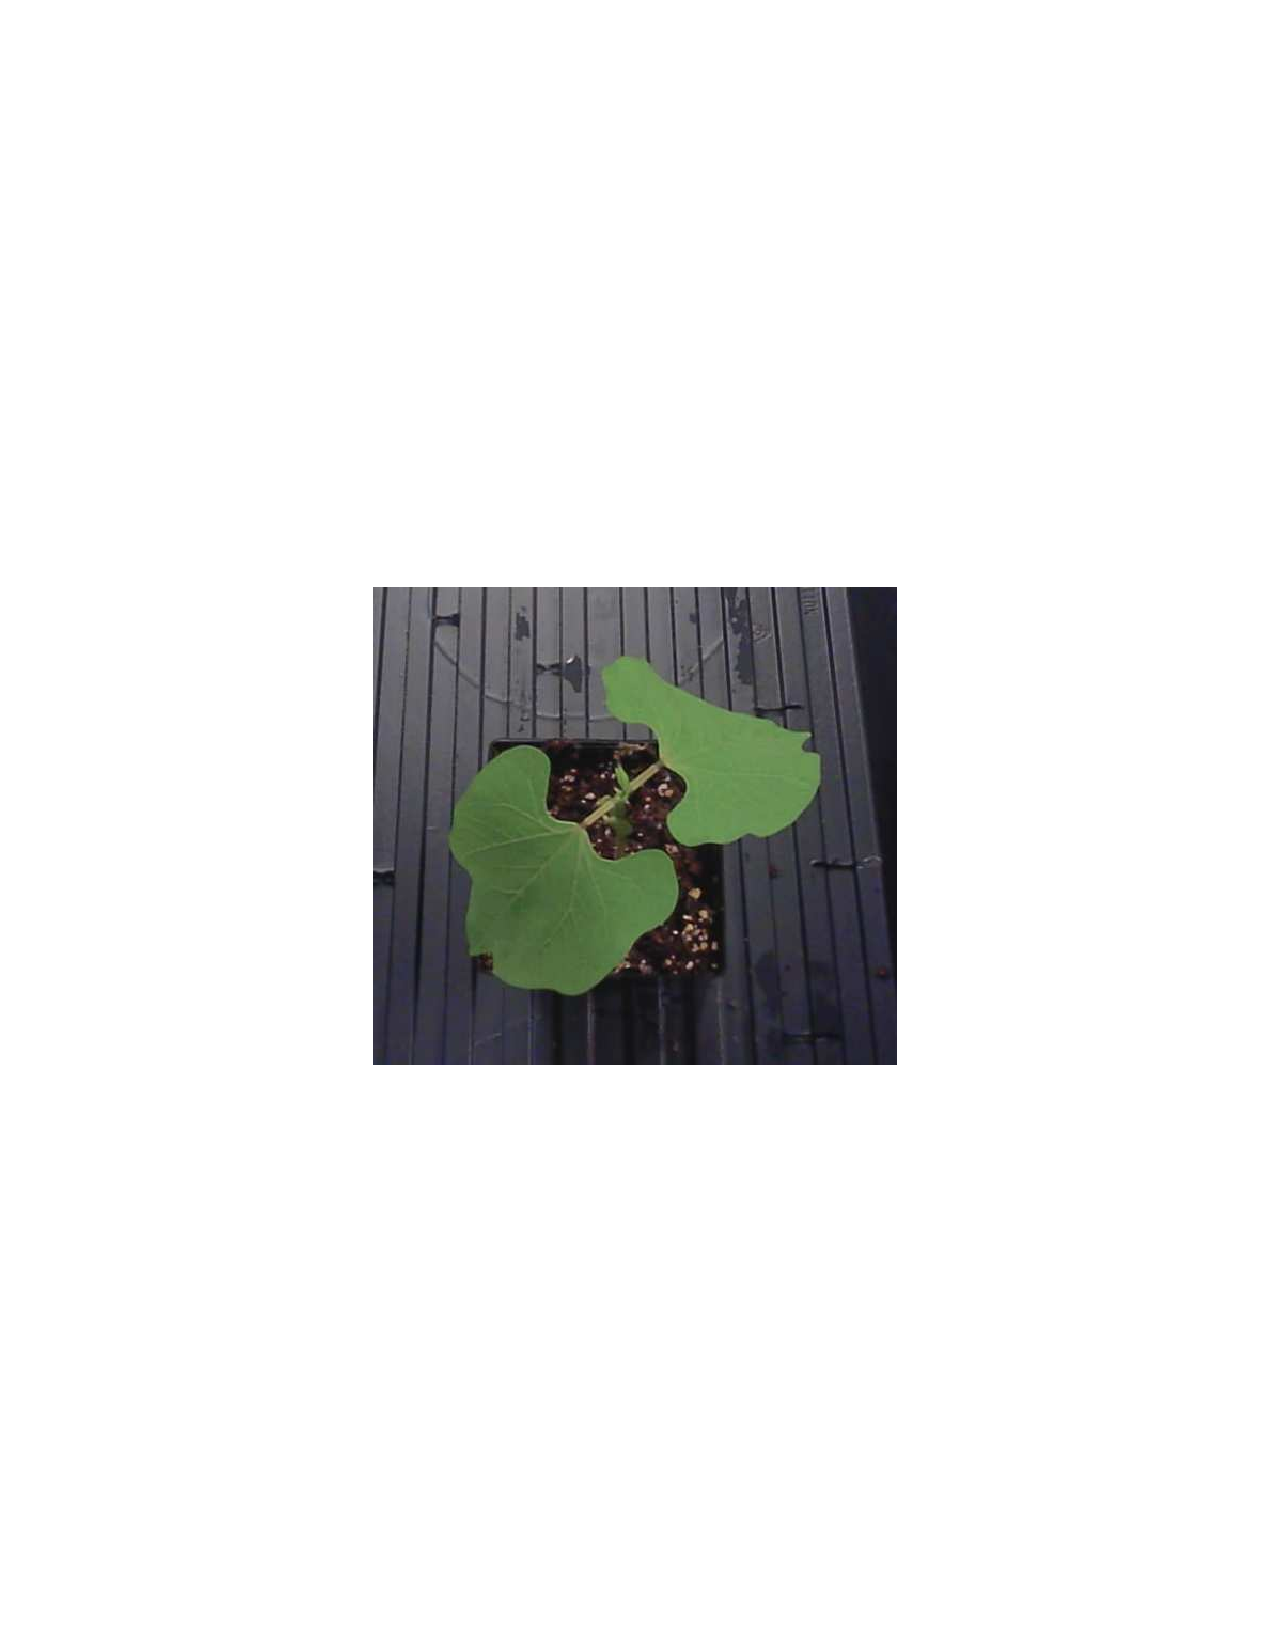
\includegraphics[trim=190 280 190 290,clip,width=0.48\linewidth]{Figures/beanColor} &
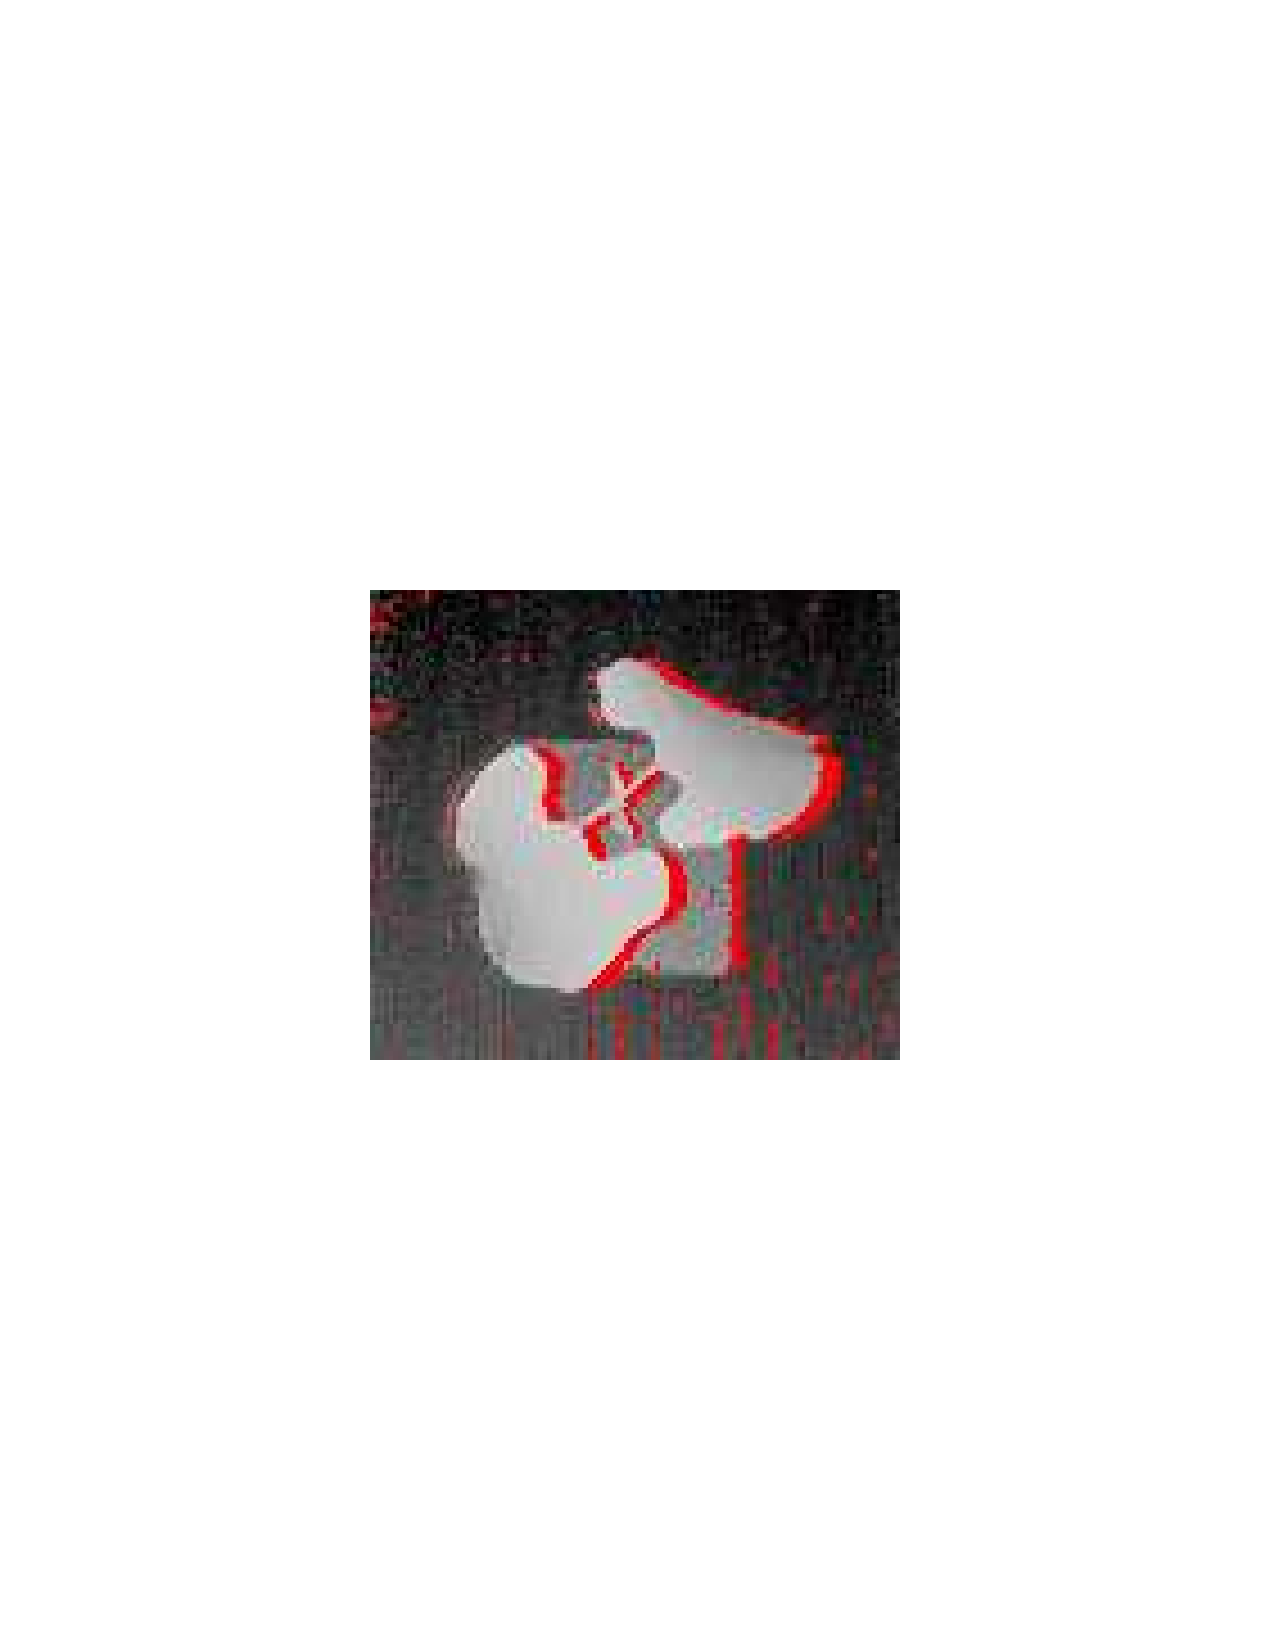
\includegraphics[trim=190 280 190 290,clip,width=0.48\linewidth]{Figures/beanDepth} \\
($a$) & ($b$) \\
%Put bead SLIC and boundary here:
($c$) & ($d$) \\
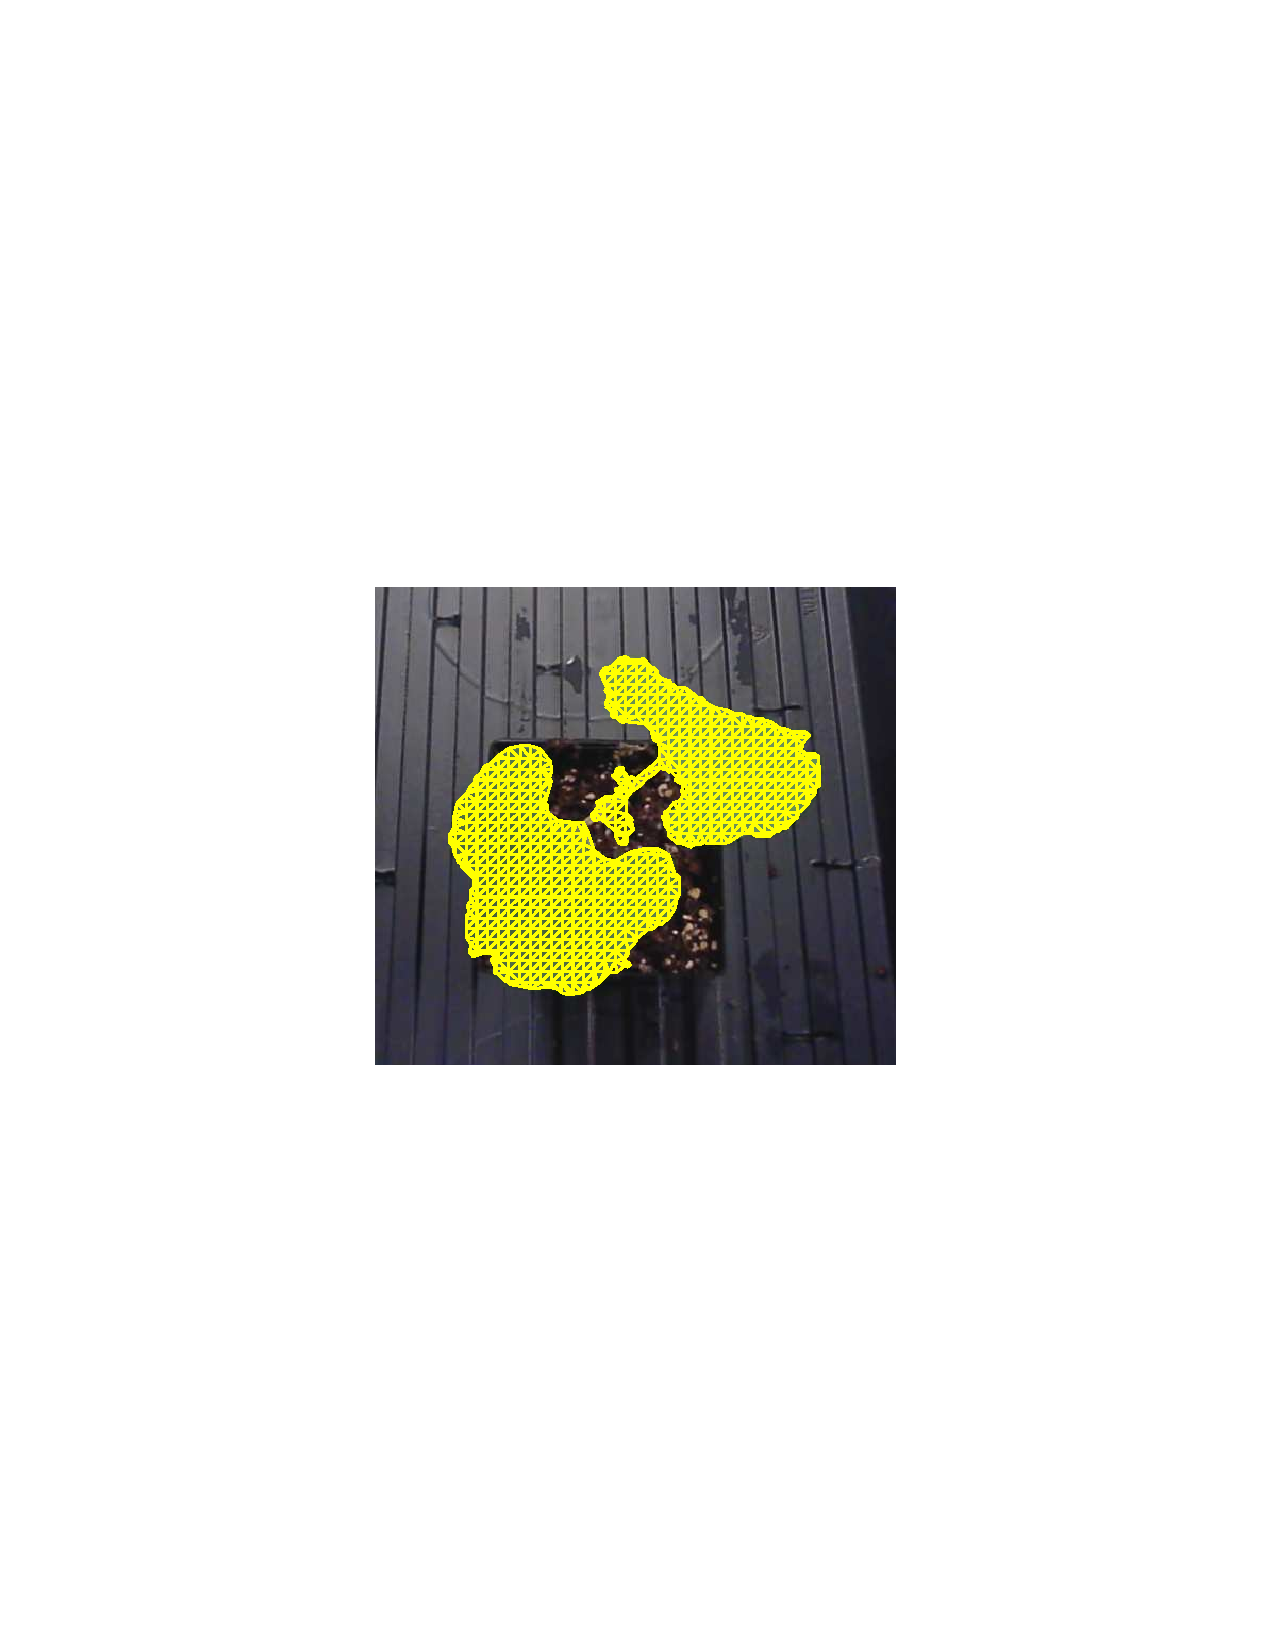
\includegraphics[trim=190 280 190 290,clip,width=0.48\linewidth]{Figures/beanColorMesh} &
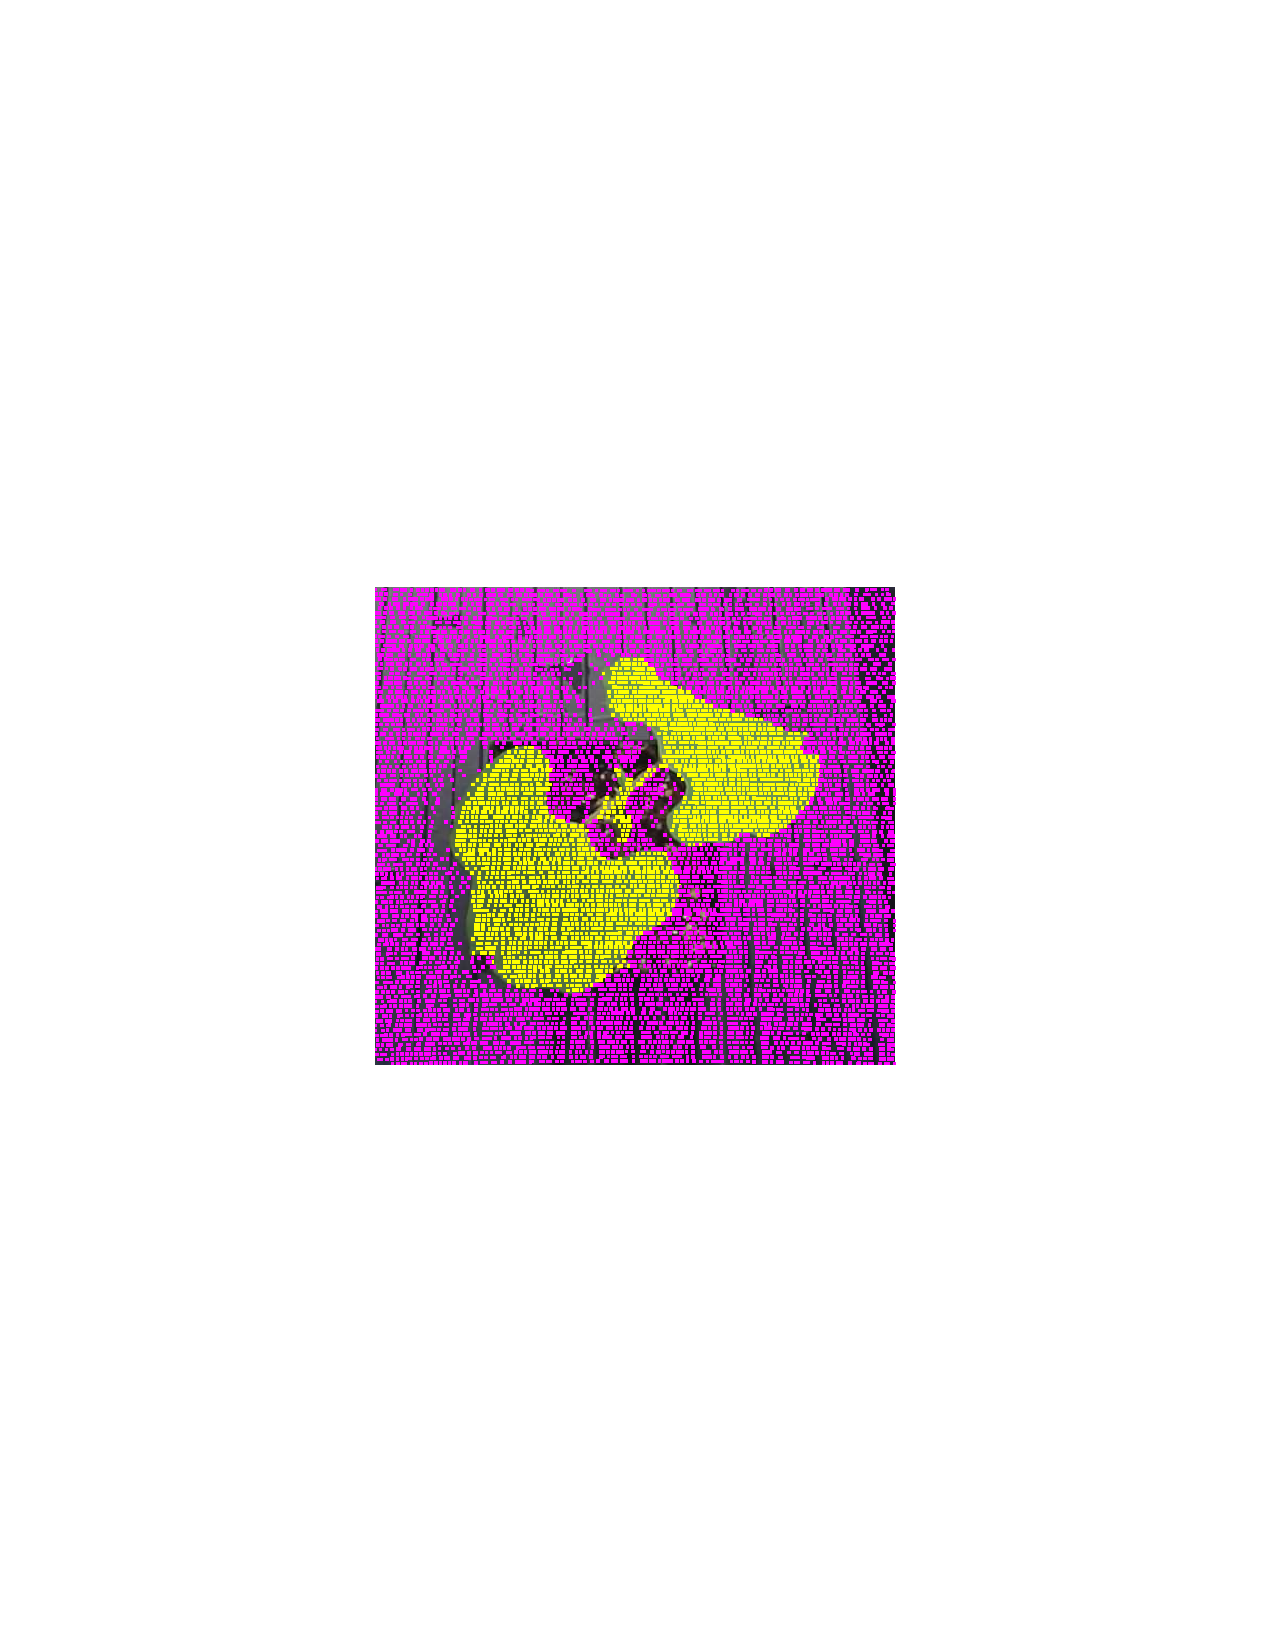
\includegraphics[trim=190 280 190 290,clip,width=0.48\linewidth]{Figures/beanPointsOnLeaves} \\
($e$) & ($f$) \\
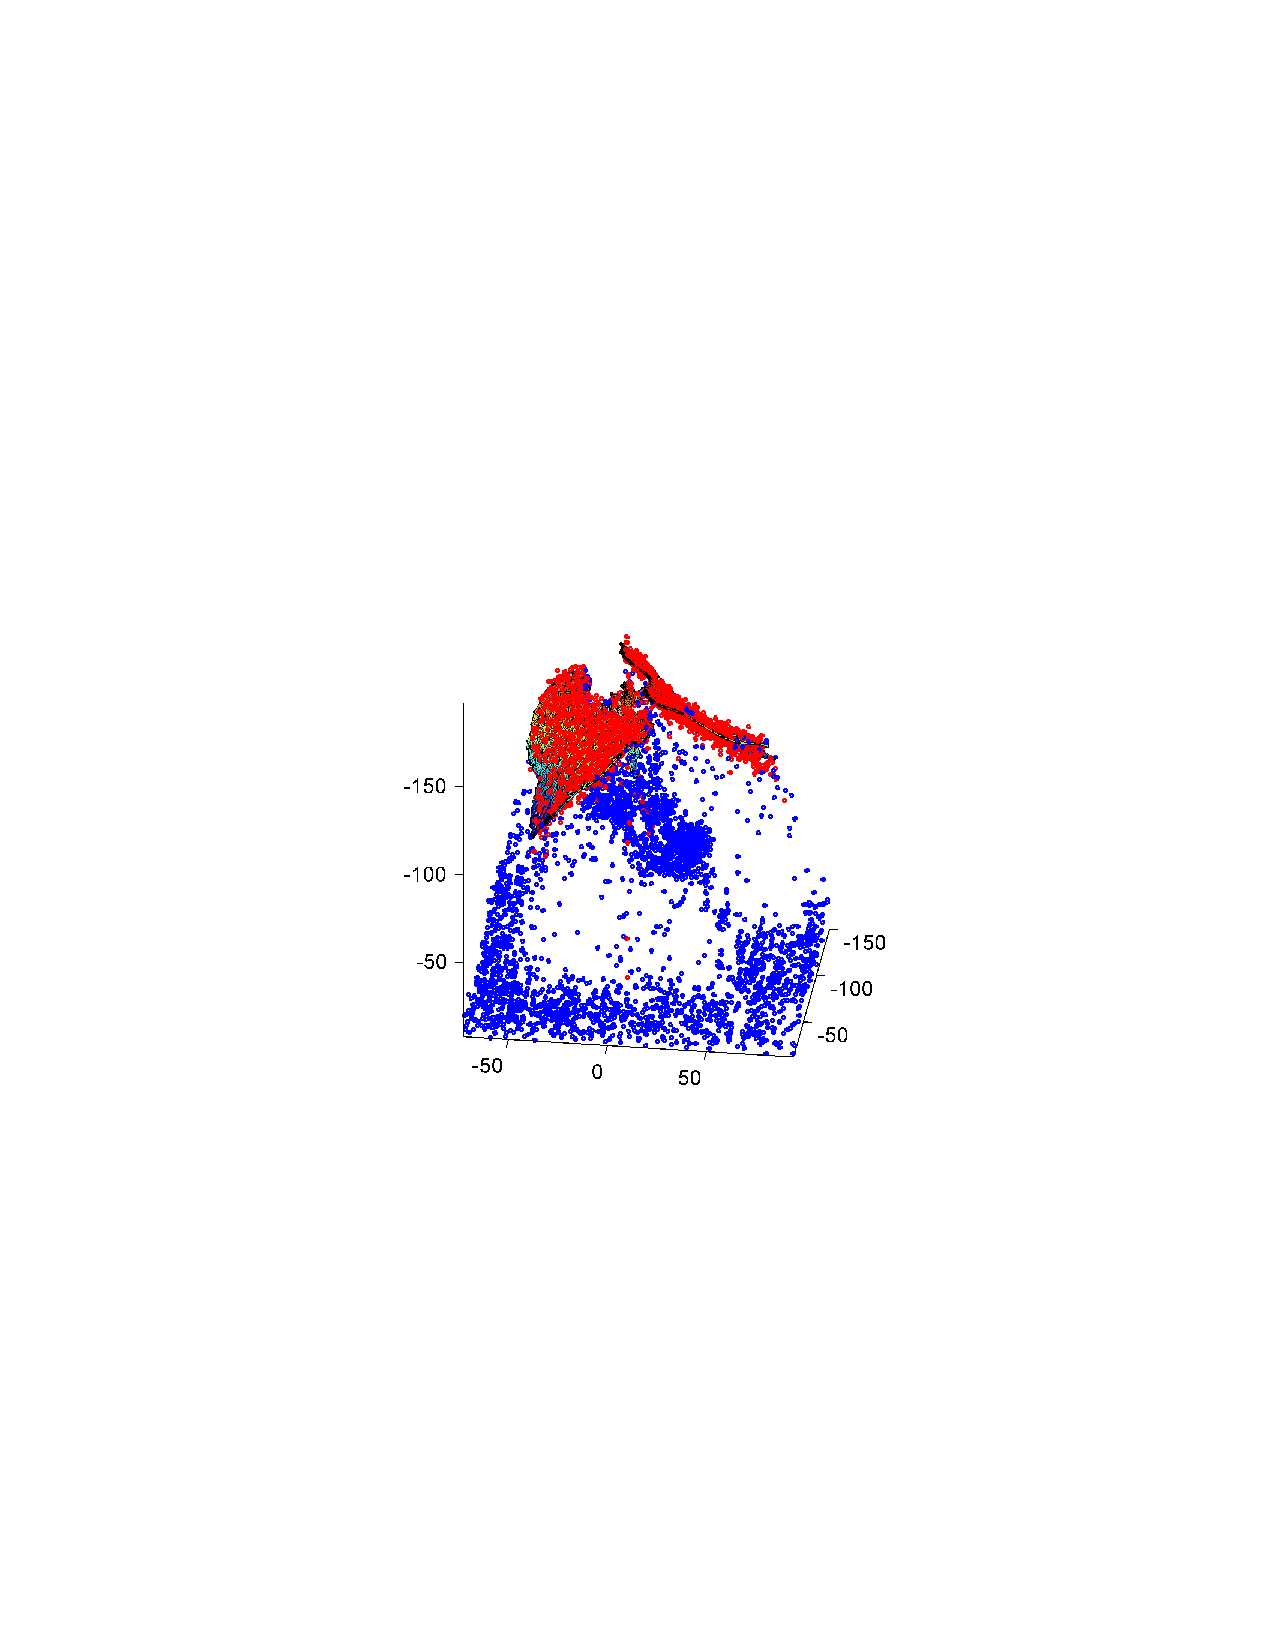
\includegraphics[trim=190 280 190 290,clip,width=0.48\linewidth]{Figures/bean3DMeshPlusPoints} &
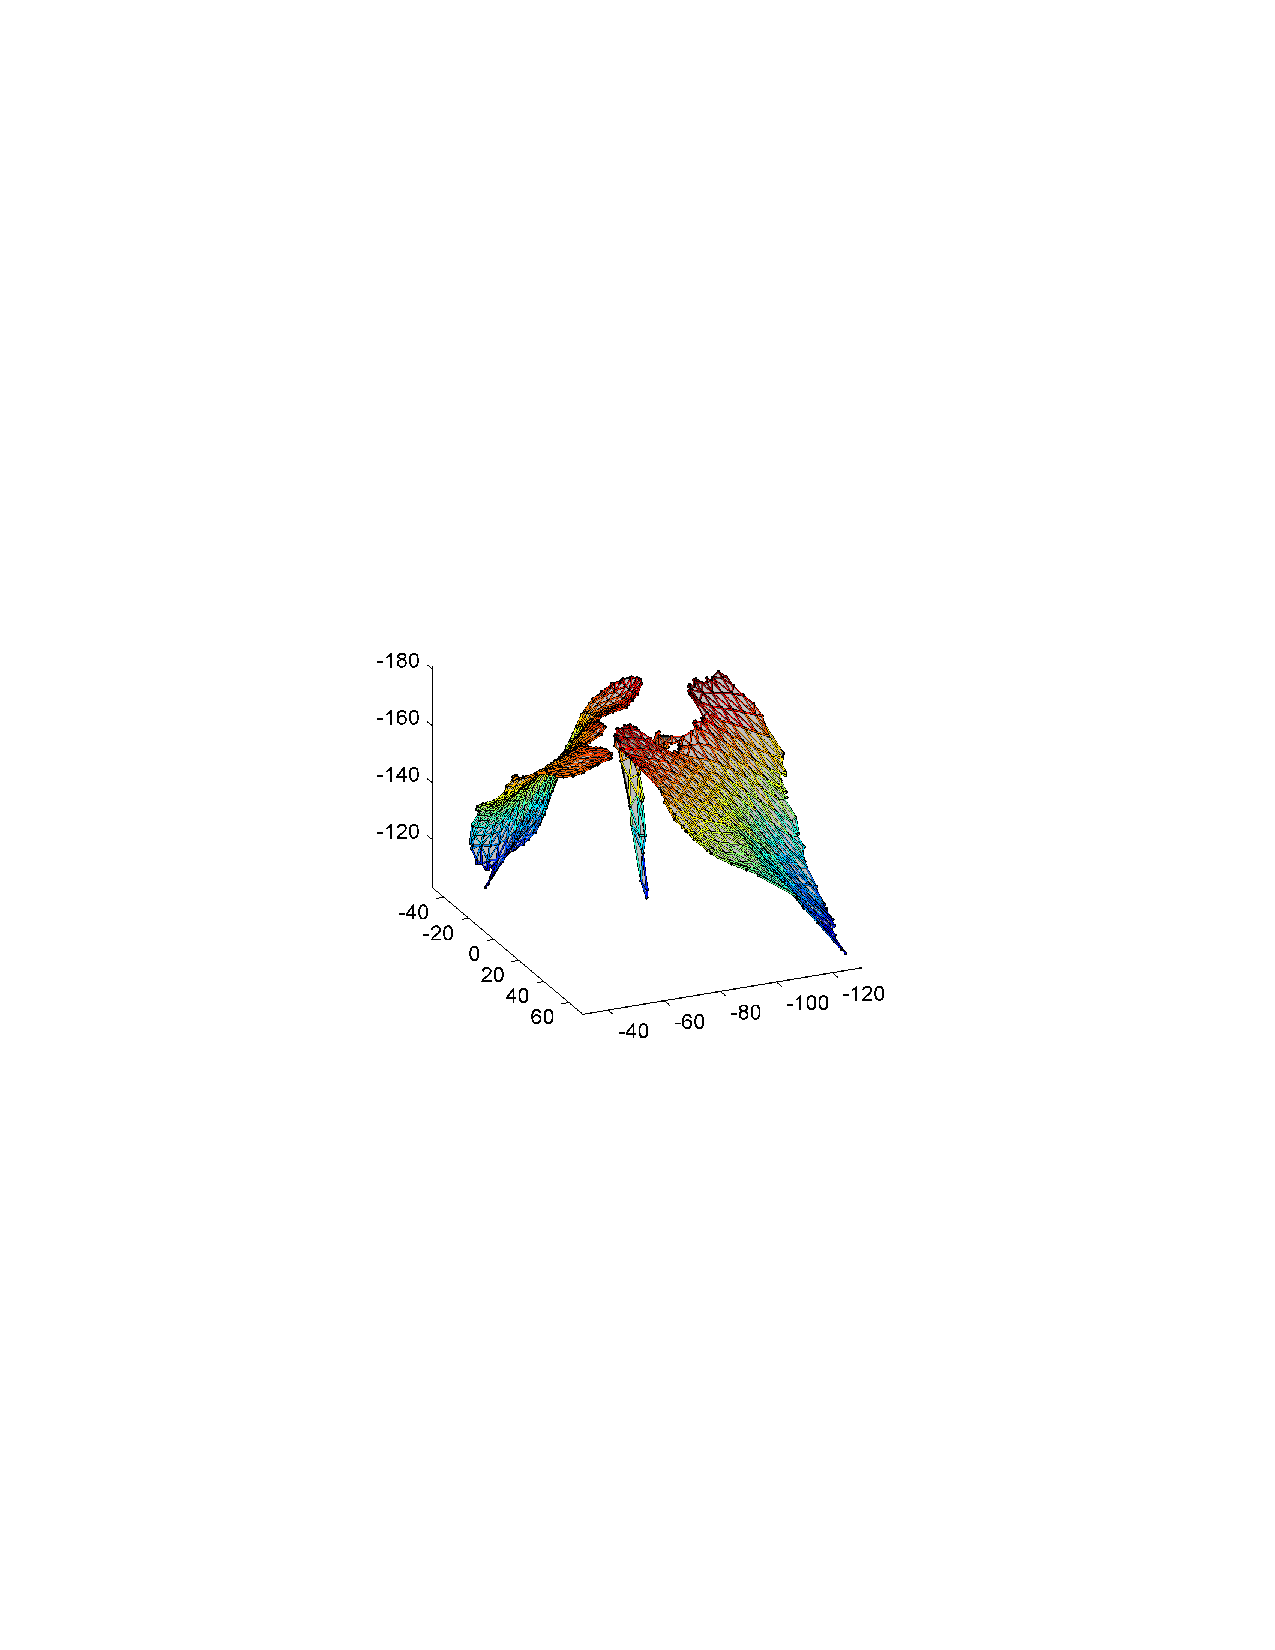
\includegraphics[trim=190 280 190 290,clip,width=0.48\linewidth]{Figures/bean3DMesh} \\
($g$) & ($h$) \\
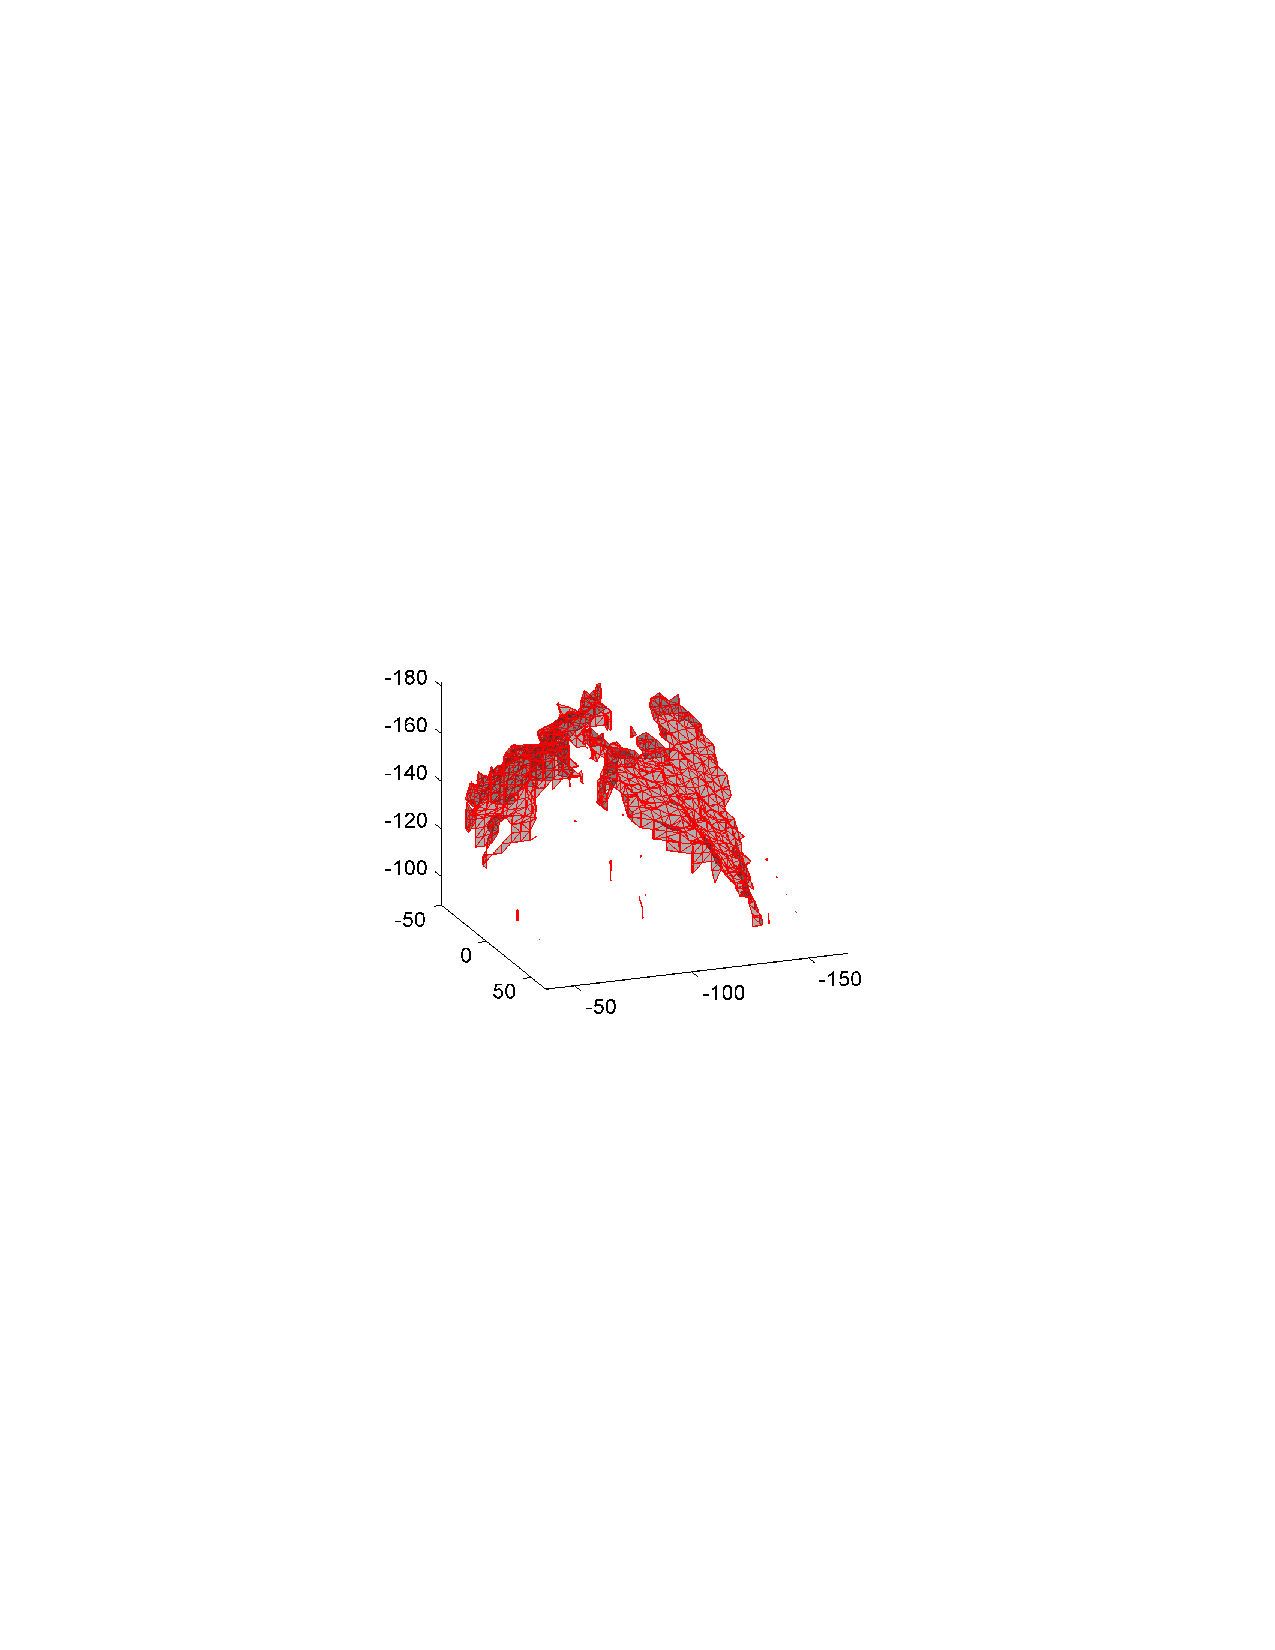
\includegraphics[trim=190 280 190 290,clip,width=0.48\linewidth]{Figures/bean3DIsosurface} & \\
($i$) & ($h$) \\
\end{tabular}
\end{center}
   \caption{The algorithm steps are illustrated.  ($a$) Color image portion on plant.  ($b$) Depth image, where red pixels are those that are masked out using the method in Fig.~\ref{fig:occlusion} as they are not visible in the color image. ($c$) ($d$), ($e$) An mesh is defined in the color image within the leaf boundaries. ($f$) Points that project into the image-mesh, excluding occluded points from ($b$), are shown in yellow over the color image, and the remaining visible points are plotted in magenta.  ($g$) The mesh fit along the vertex rays is shown.  The $3$D points are red for those on the mesh and blue for the remaining.  ($h$) A more detailed view of the mesh. ($i$) A comparison with an isosurface created using marching cubes~\cite{} }
\label{fig:sigmainterframe}
\end{figure}


\begin{figure}
\begin{center}
\begin{tabular}{cc}
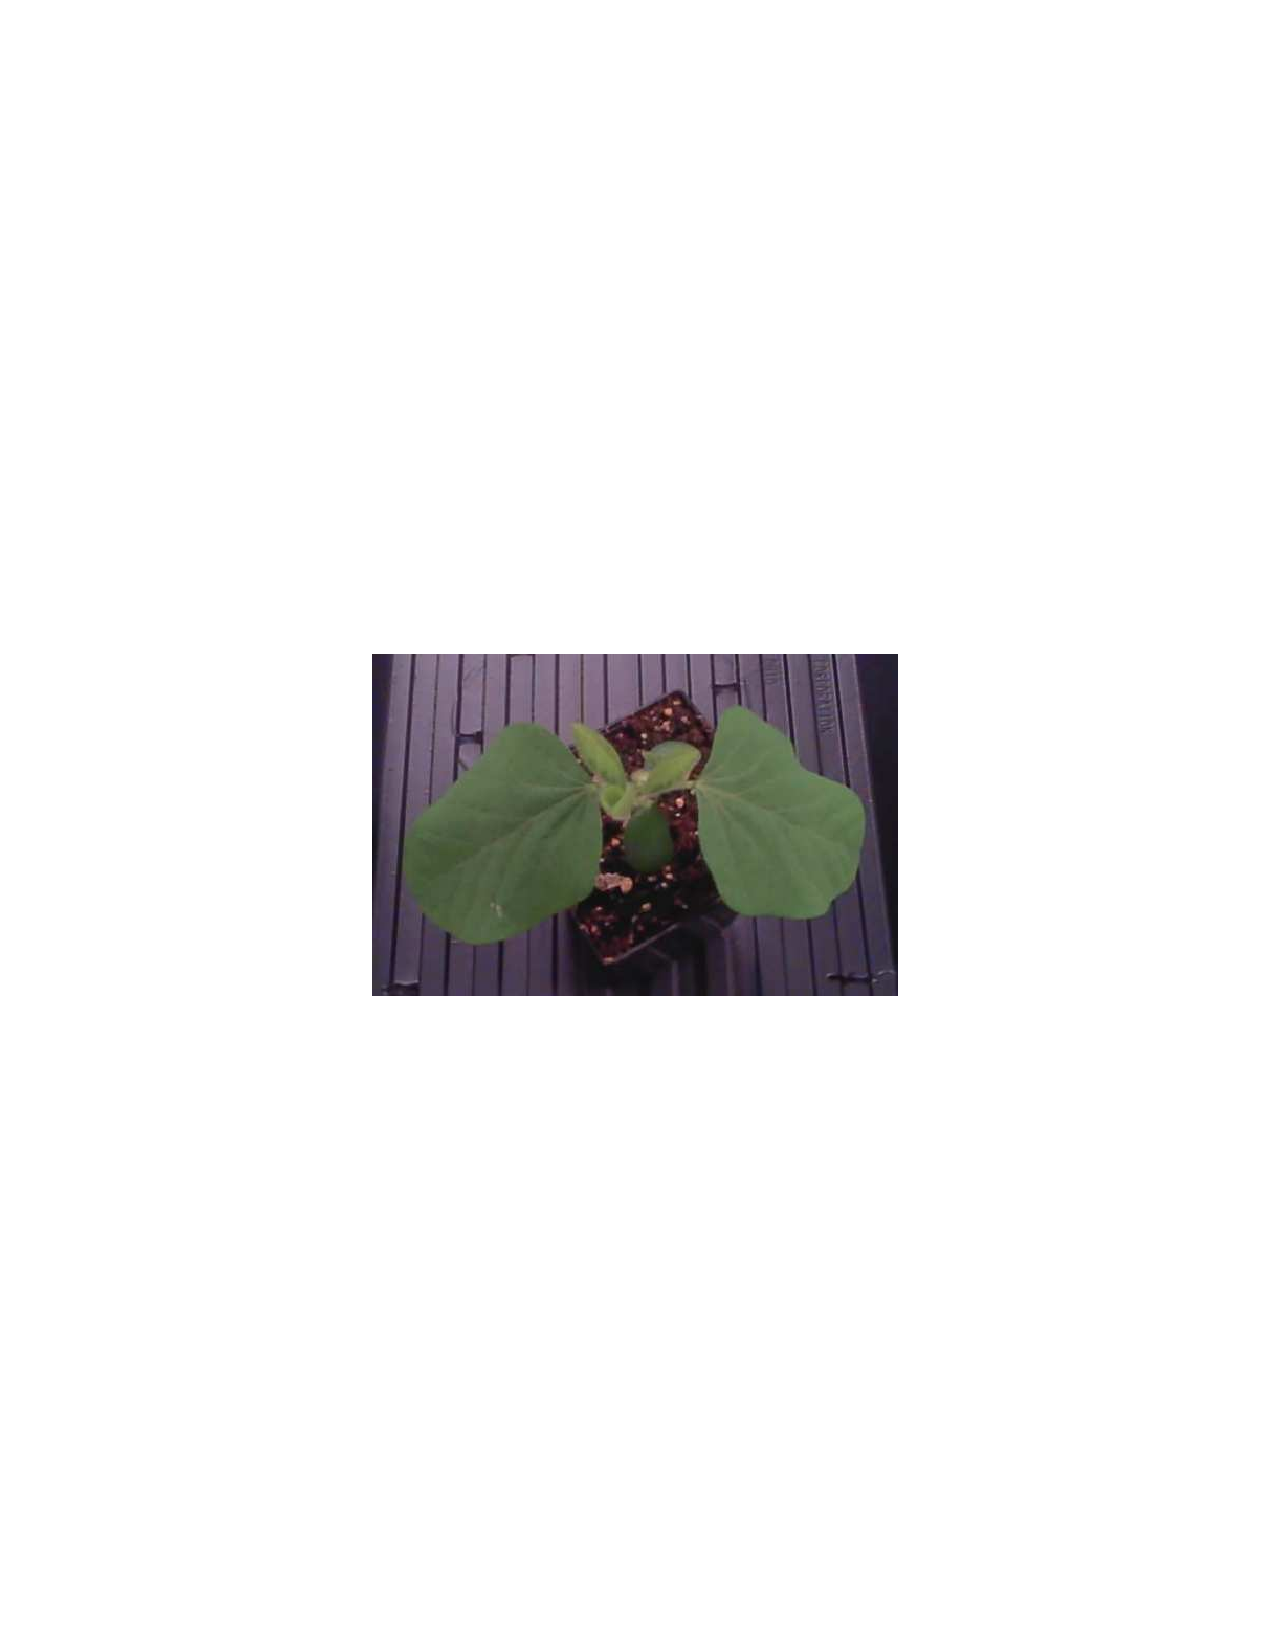
\includegraphics[trim=190 280 190 290,clip,width=0.48\linewidth]{Figures/soybeanColor} &
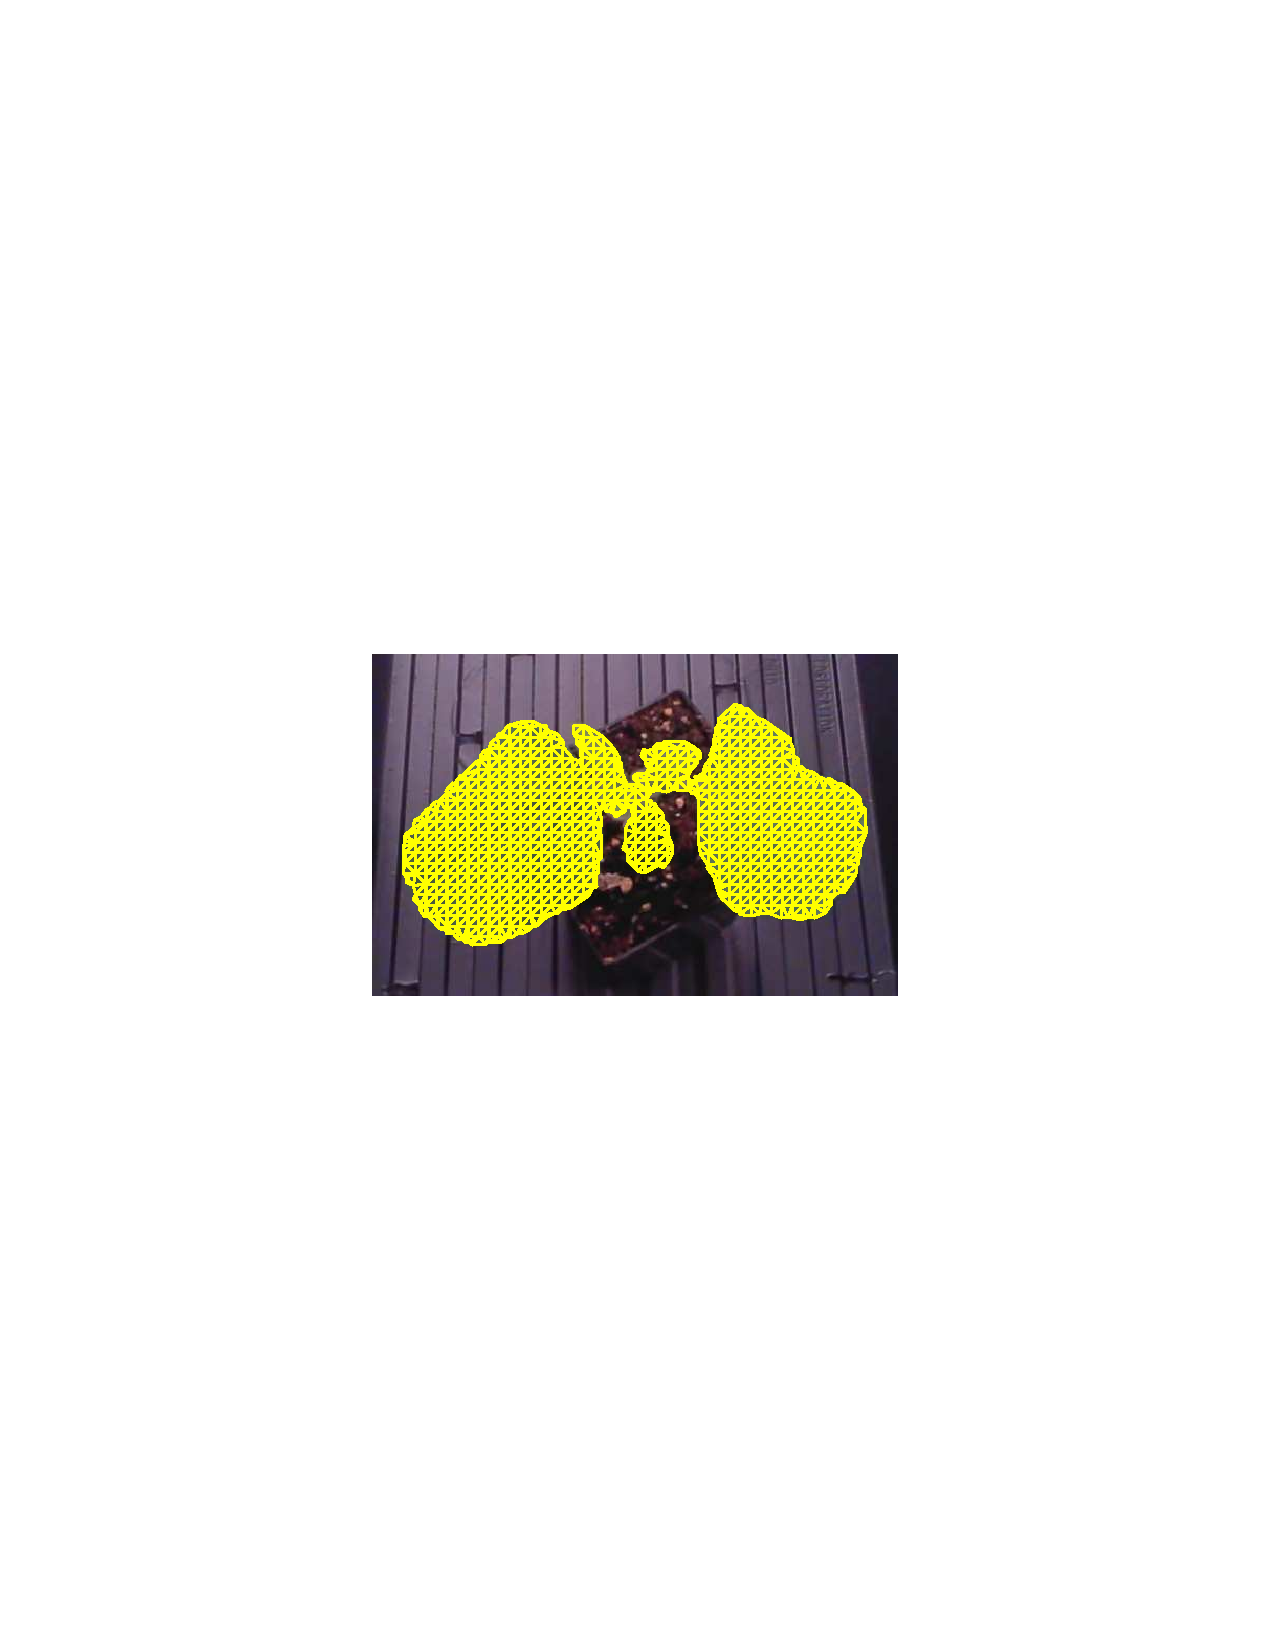
\includegraphics[trim=190 280 190 290,clip,width=0.48\linewidth]{Figures/soybeanColorMesh} \\
($a$) & ($b$) \\
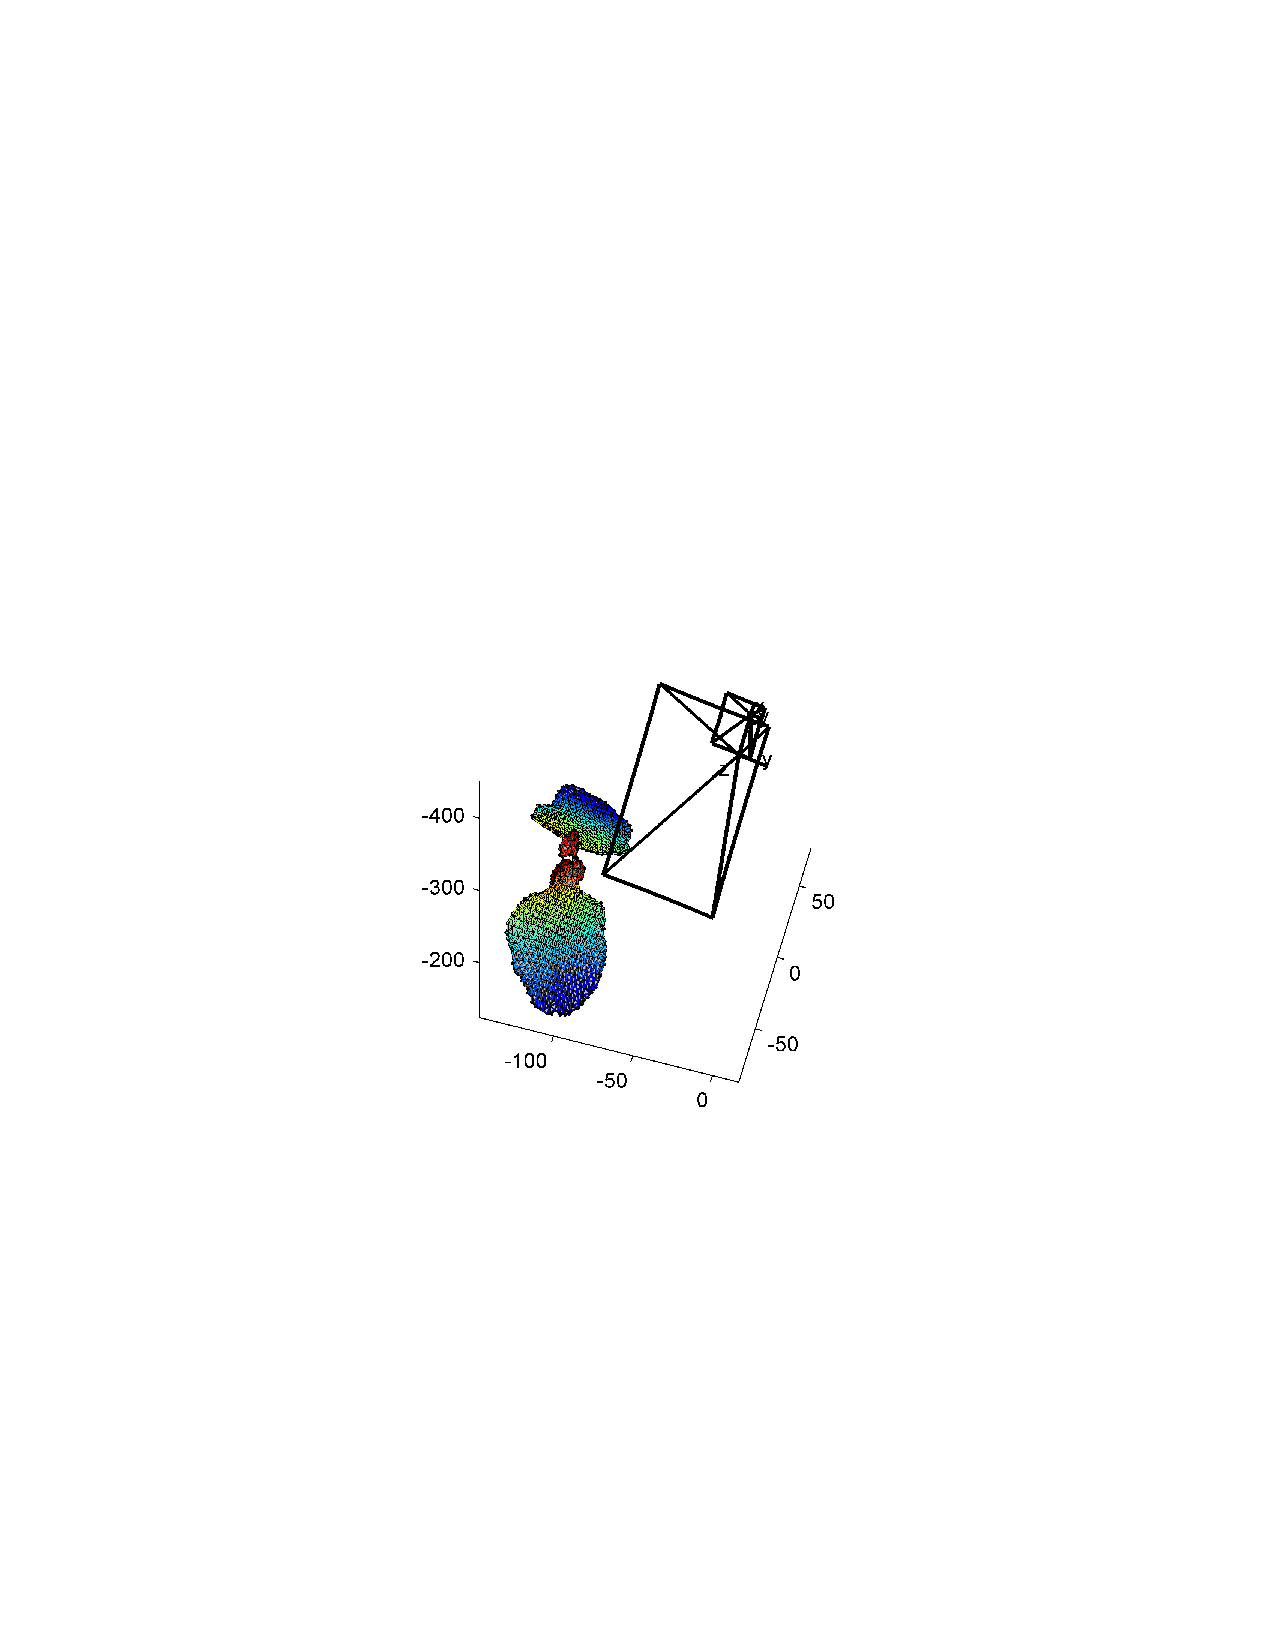
\includegraphics[trim=190 280 190 290,clip,width=0.48\linewidth]{Figures/soybean3DMeshPlusCam} &
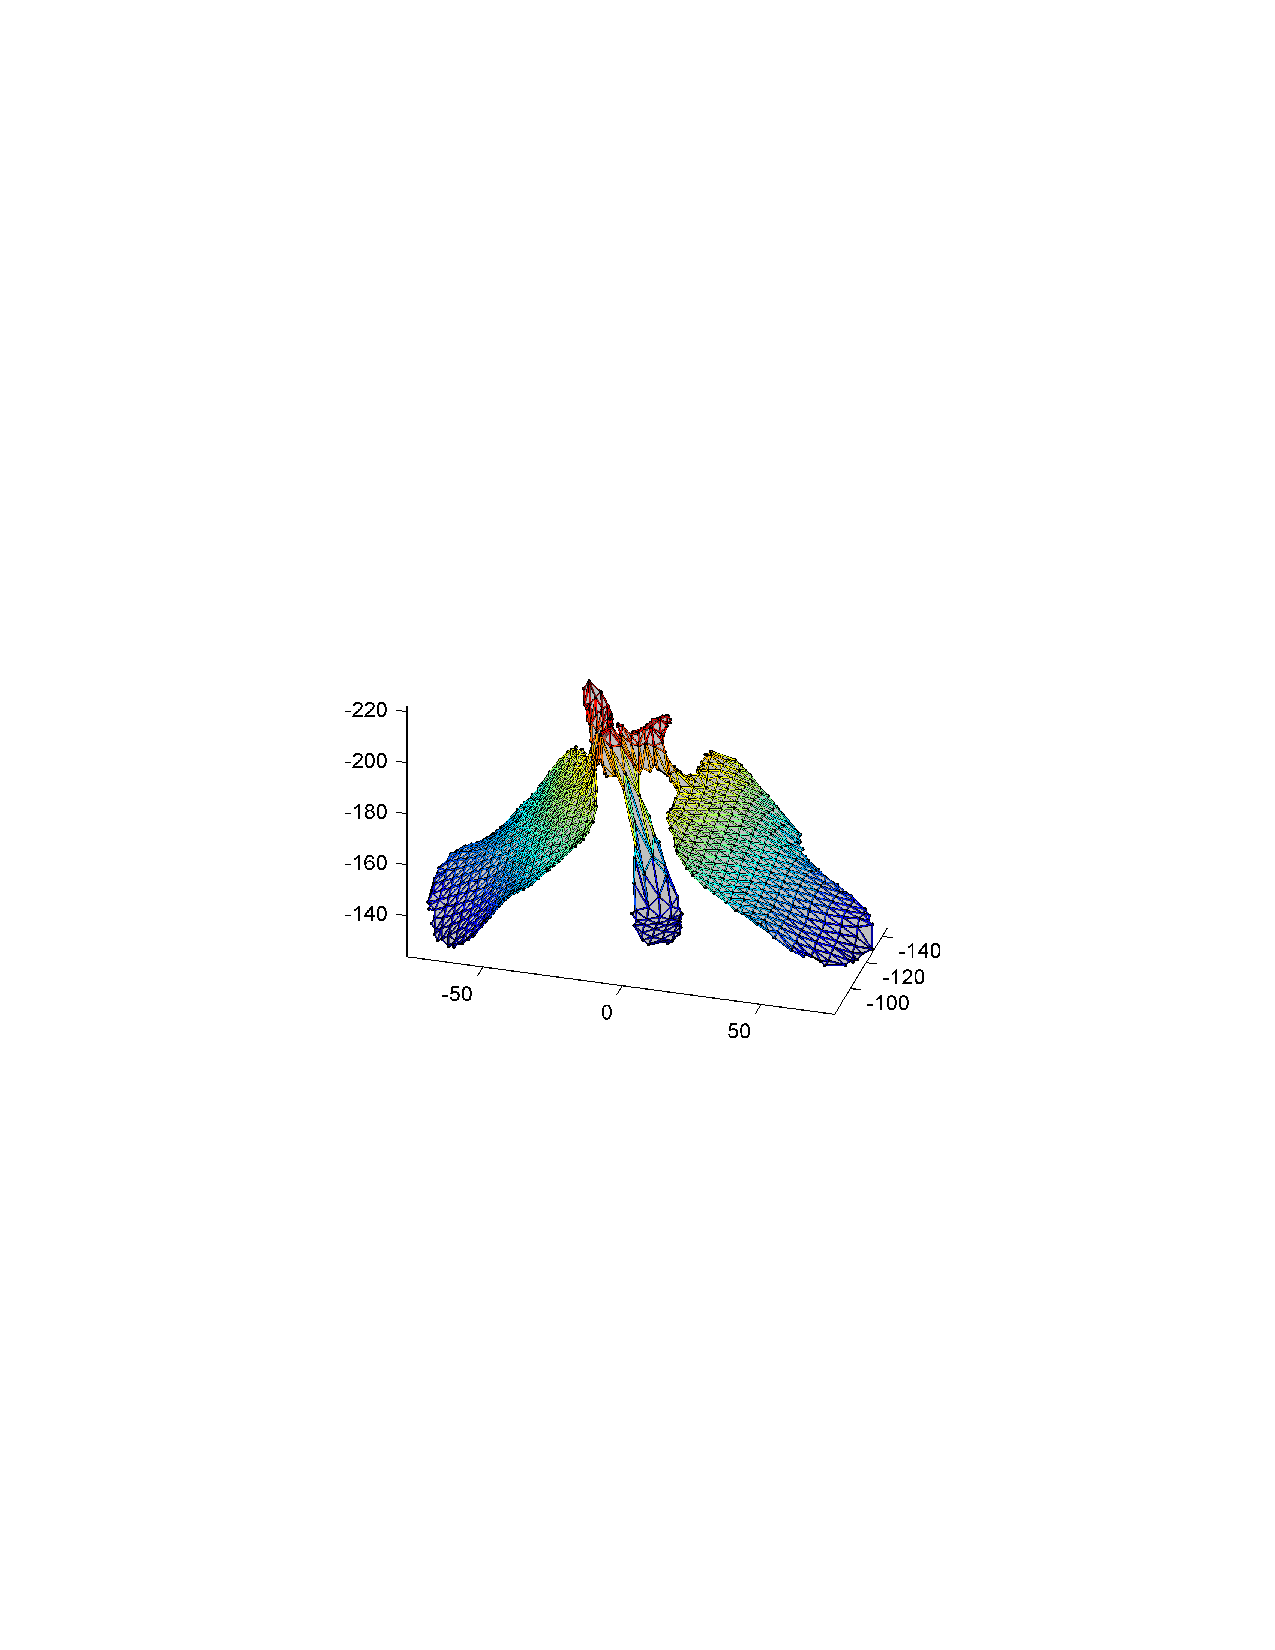
\includegraphics[trim=190 280 190 290,clip,width=0.48\linewidth]{Figures/soybean3DMesh} \\
($c$) & ($d$) \\
\end{tabular}
\end{center}
   \caption{($a$) Color image of a soybean plant.  ($b$) Mesh on the color image. ($c$) $3$D mesh along with camera poses. ($d$) Close-up of $3$D mesh.  }
\label{fig:sigmainterframe}
\end{figure}



